% !TEX root = ../00_tcc.tex

\begin{figure}[H]
	\centering
	\begin{subfigure}[b]{\textwidth}
		\centering
		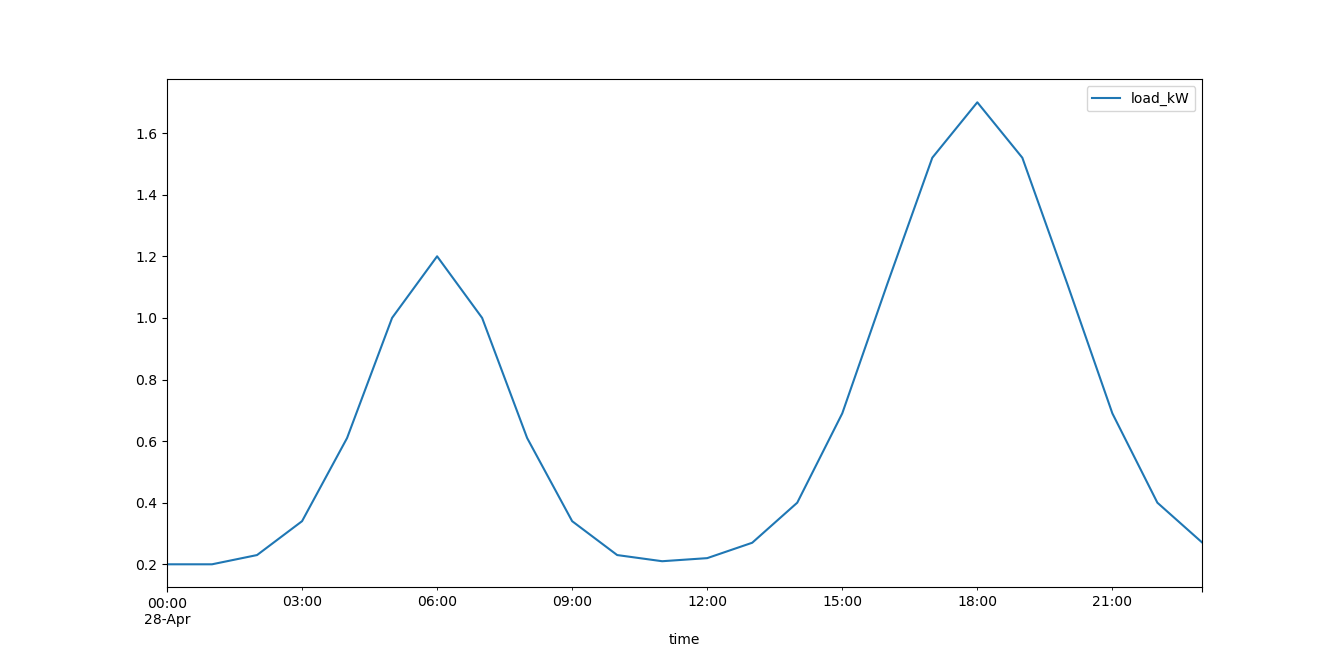
\includegraphics[width=0.7\textwidth]{../img/load.png}
		\caption{Curva original}\label{fig:load}
	\end{subfigure}
	\\ \vspace{0.1cm}
	\begin{subfigure}[b]{\textwidth}
		\centering
		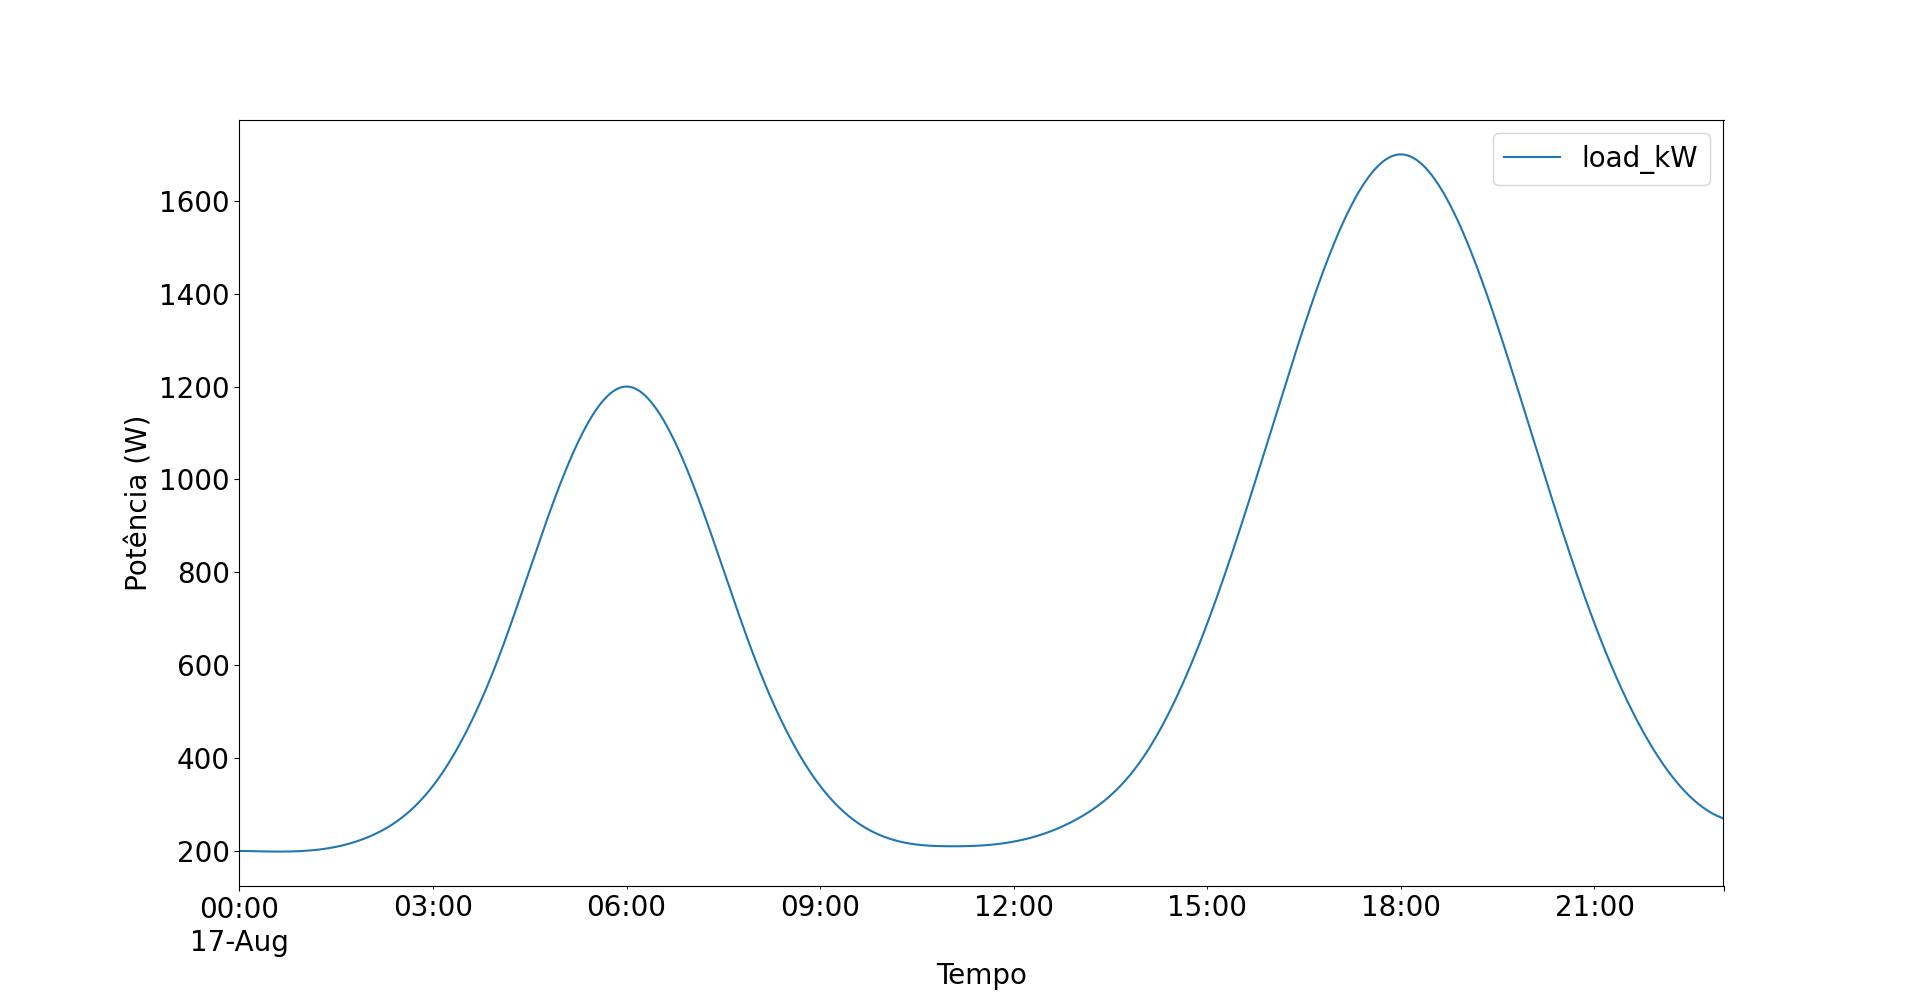
\includegraphics[width=0.7\textwidth]{../img/load_corr.png}
		\caption{Curva interpolada}\label{fig:load_corr}
	\end{subfigure}
	\caption{Perfil de carga de exemplo. Fonte: própria.}\label{fig:perfil}
\end{figure}
